% ==================== CHAPTER 1: PRELIMINARY STUDY ====================
% ==================== SECTION NUMBERING RULE ====================
% Section numbering DOES NOT include chapter number.
% After chapter introduction, first section is numbered 1. (not 1.1 or 2.1)
% Then subsequent subsections are numbered 1.1, 1.2, 1.3, etc.
% Following sections reset to 2., 2.1, 2.2, etc. within the same chapter.
% ============================================================================
% STYLE GUIDELINES FOR ALL CHAPTERS:
% - Each chapter starts on a new page with title page
% - Font: Times New Roman 12pt for body, line spacing 1.5
% - Titles: Left-aligned, numbered decimally (1, 1.1, 1.1.1), bold
% - No title isolated at bottom of page (avoid orphans/widows)
% - If a section has subsections, add a short descriptive paragraph immediately after the parent heading before the first subsection.
% - Figures/Tables: Numbered consecutively (Figure 1.1, Table 1.1, etc.)
% - Figure captions: Below figure, 12pt Times, centered, justified
% - Table captions: Above table, 12pt Times, centered, justified
% - One blank line above caption, two blank lines below
% - Formulas: Numbered (1) to (n), right-aligned
% - Emphasis: Use italics or bold, NEVER underline
% - No automatic hyphenation
% 
% CHAPTER 1 CONTENT:
% - General project context (Novation City and academic framework)
% - Problem statement and study of existing solutions
% - Proposed solution and requirements specification
% - Agile Scrum methodology and project planning
% ============================================================================
% ==================== CHAPTER 1: PRELIMINARY STUDY ====================
\chapter{Preliminary Study}
\setcounter{section}{0}

\section*{Introduction}
\addcontentsline{toc}{section}{Introduction}

\initial{T}his chapter presents the preliminary study of the IoT-REAP project. It situates the work in the Novation City context, reviews existing industrial remote access solutions, defines the proposed platform and its requirements, and ends with the methodology and planning used to structure the implementation.

\section{General Project Context}

Novation City serves as the professional context for the IoT-REAP platform development. This section situates the project within the cluster's institutional framework, business units, infrastructure, and academic setting, all of which explain why a secure remote industrial access platform was needed.

\subsection{Host Organization}

Novation City is a competitiveness cluster established in 2009 in Sousse, Tunisia, as a public-private partnership. The cluster is designed to foster innovation ecosystems and enhance industrial competitiveness through digital transformation and advanced technologies, addressing the growing need for mechatronics expertise and Industry 4.0 adoption in the MENA region \cite{novationcity2025}.

\begin{figure}[H]
\centering

\includegraphics[width=3.5cm]{assets/chapter1/novation-city-logo.png}
\caption{Novation City Official Logo and Branding}
\label{fig:novation-logo}
\end{figure}

\textbf{Mission Statement:} Novation City's mission is to foster an innovation ecosystem in the mechatronics sector by synergizing innovative companies, industrial entities, research centers, universities, and engineering schools. The cluster aims to enhance regional and national competitiveness through technology advancement, knowledge transfer, and strategic investment attraction.

\textbf{Vision:} The cluster envisions becoming the leading competitiveness hub for Industry 4.0 adoption and digital transformation in North Africa and the broader MENA region, focusing on world-class innovation infrastructure, highly skilled technical talent development, and sustainable academia-industry partnerships.
\newpage
\subsection{Business Units and Services}

Novation City operates through four specialized business units, each addressing distinct aspects of the innovation ecosystem:

\textbf{Acceleration Unit:} Supports startup growth through business incubation services, mentorship programs, and access to funding opportunities. Services include workspace provision, networking, and investor connections.

\textbf{Advisory Unit:} Delivers strategic consulting focused on digital transformation and Industry 4.0 implementation. The advisory services encompass digital readiness assessment, technology selection, change management, security compliance audits, and infrastructure planning for remote operations platforms.

\textbf{Formation Unit (Novation Akademy):} Provides training and skills development programs covering mechatronics, automation, digital technologies, project management, and innovation methodologies in collaboration with universities and industry partners.

\textbf{Innovation Unit:} Drives research and development initiatives, facilitating collaborative R\&D between academic institutions and industrial partners while exploring emerging technologies for the regional ecosystem.

\subsection{Infrastructure and Strategic Focus}

Novation City manages three specialized geographic zones:

\begin{itemize}
    \item \textbf{Mechatronic City:} Houses companies focused on mechatronics, robotics, and advanced manufacturing with specialized laboratories and testing facilities.
    \item \textbf{Business City:} Accommodates service-oriented companies and consulting firms with modern office spaces and collaborative environments.
    \item \textbf{Industrial City:} Dedicated to manufacturing operations with infrastructure supporting advanced manufacturing processes and Industry 4.0 technologies.
\end{itemize}

A central pillar of Novation City's strategy is promoting Industry 4.0 principles and digital transformation. The cluster recognizes that many industrial companies face significant challenges in implementing Industry 4.0 technologies, including limited awareness, uncertainty about ROI, skills gaps, and integration difficulties with legacy systems.

To address these challenges, Novation City extends its capabilities with secure remote access platforms enabling engineers to interact with industrial systems remotely through the IoT-REAP initiative, combining Infrastructure-as-a-Service provisioning with zero-trust security principles \cite{edb2017} \cite{tuvsud2023}.

\subsection{Academic Framework}

This project was carried out as part of an internship report in a software engineering and Industry 4.0 context. The academic objective was to apply web engineering, software architecture, database modeling, remote infrastructure integration, and secure system design to a real industrial problem. The work also required formal documentation through UML modeling, requirements analysis, implementation reporting, and verification of the delivered platform.

\subsection{Problem Statement}

The IoT-REAP project emerges from critical operational challenges facing industrial companies and training institutions within the Industry 4.0 ecosystem. As manufacturing systems become increasingly digitized and interconnected, engineers and technicians require hands-on access to specialized industrial equipment—PLCs (Programmable Logic Controllers), HMIs (Human-Machine Interfaces), SCADA systems, and industrial robots—for training, development, and maintenance purposes.

\textbf{Remote Access Limitations:} Traditional approaches to industrial system access present significant challenges:

\begin{itemize}
    \item Physical presence requirements limit training scalability and increase travel costs
    \item VPN-based solutions are complex to configure, difficult to maintain, and often incompatible with OT (Operational Technology) security requirements
    \item Existing remote desktop tools lack integration with industrial protocols and equipment
    \item No unified platform exists for VM provisioning, remote desktop access, and IoT device control
\end{itemize}

\textbf{Security Concerns in OT Environments:} Industrial networks require strict isolation following the Purdue model, yet traditional IT remote access tools are not designed for OT security requirements:

\begin{itemize}
    \item \textbf{Network Segmentation:} IT remote access solutions often bypass OT network boundaries, creating security vulnerabilities
    \item \textbf{Session Management:} No automatic session expiration or quota management for shared industrial resources
    \item \textbf{Audit Trail:} Insufficient logging for compliance with industrial security standards (IEC 62443)
    \item \textbf{Access Control:} Lack of fine-grained role-based access to different industrial zones
\end{itemize}

\textbf{Resource Sharing Challenges:} Educational institutions and industrial companies face difficulties in sharing expensive equipment:

\begin{itemize}
    \item \textbf{Equipment Scarcity:} Industrial robots and specialized VMs are costly and limited in quantity
    \item \textbf{Scheduling Conflicts:} No automated reservation system prevents double-booking of shared resources
    \item \textbf{Utilization Monitoring:} Inability to track usage patterns and optimize resource allocation
    \item \textbf{Maintenance Visibility:} No predictive maintenance for shared industrial equipment
\end{itemize}

\begin{table}[H]
\centering
\caption{Critical Limitations of Current Industrial Remote Access Solutions}
\begin{tabular}{|p{3.5cm}|p{5.5cm}|p{5cm}|}
\hline
\textbf{Limitation Category} & \textbf{Specific Problem} & \textbf{Business Impact} \\
\hline
Physical Access & Engineers must be on-site to access equipment & Limited training capacity, high travel costs \\
\hline
VPN Complexity & Complex configuration, security vulnerabilities & IT overhead, OT security risks \\
\hline
Fragmented Tools & Separate systems for VMs, remote desktop, robots & Context-switching, integration difficulties \\
\hline
No Session Management & No automatic expiration or resource quotas & Resource conflicts, security exposure \\
\hline
Limited Audit Trail & Insufficient logging for compliance & IEC 62443 non-compliance \\
\hline
No Predictive Maintenance & Reactive maintenance only & Equipment downtime, safety risks \\
\hline
\end{tabular}
\label{tab:current-limitations}
\end{table}

\section{Study of the Existing}

Before proposing the IoT-REAP architecture, it is essential to examine current
industrial remote access solutions, understand their technical approaches, and
identify the specific gaps they fail to address. This analysis establishes the
foundation for the proposed platform design.

\subsection{Analysis of Existing Industrial Remote Access Solutions}

Industrial remote access has traditionally relied on several established
approaches, each with distinct characteristics and limitations. Understanding
these existing solutions is essential for positioning the IoT-REAP platform
within the current technological landscape.

\textbf{Virtual Private Networks (VPNs):} The most common approach for industrial remote access involves establishing encrypted tunnels between remote users and industrial networks. Organizations deploy VPN concentrators at facility perimeters, requiring engineers to install client software, configure connections, and authenticate before accessing internal resources.

\textbf{Jump Servers / Bastion Hosts:} Some organizations implement intermediate servers that act as controlled access points to OT networks. Engineers first connect to the jump server, then establish secondary connections to target systems. This adds a security layer but increases connection complexity and latency.

\textbf{Proprietary Remote Access Tools:} Industrial equipment vendors (Siemens, Rockwell, Schneider) offer vendor-specific remote access solutions tied to their hardware ecosystems. These tools provide optimized connections to specific PLCs and HMIs but create vendor lock-in and fragmentation across multi-vendor environments.

\textbf{Cloud-Based IIoT Platforms:} Emerging platforms like AWS IoT, Azure IoT Hub, and PTC ThingWorx provide cloud connectivity for industrial devices. However, these focus primarily on data collection and monitoring rather than interactive remote control and desktop access.

\textbf{Generic Remote Desktop Solutions:} Tools like TeamViewer, AnyDesk, and Microsoft RDP provide remote desktop capabilities but lack industrial-specific features such as OT network isolation, session quotas, audit logging for compliance, and integration with virtualization platforms.

\subsection{Criticism of the Existing}

The current industrial remote access landscape exhibits several fundamental
deficiencies:

\textbf{VPN Complexity and Security Risks:} VPN deployments require significant IT expertise for configuration and maintenance. Split tunneling creates security vulnerabilities, and VPN credentials are prime targets for attackers. Once inside the VPN, lateral movement across the network is often unrestricted, violating zero-trust principles.

\textbf{Lack of Session Management:} Existing solutions provide no automated session expiration, resource quotas, or reservation systems. Shared equipment (industrial VMs, robots) cannot be efficiently scheduled, leading to conflicts and underutilization.

\textbf{No OT/IT Network Isolation:} Traditional remote access tools do not enforce Purdue model network segmentation. Engineers accessing OT systems from IT networks create security vulnerabilities that violate IEC 62443 standards.

\textbf{Missing Audit Trail:} Compliance with industrial security standards requires comprehensive logging of all access and commands. Existing tools lack tamper-proof audit logs with cryptographic integrity verification.

\textbf{Fragmented Tooling:} Organizations must deploy separate systems for VM management, remote desktop, IoT device control, and camera monitoring. This fragmentation increases operational complexity and prevents unified security policies.

\textbf{No Predictive Capabilities:} Existing solutions provide no demand forecasting for resource allocation or predictive maintenance for connected equipment. Administrators cannot anticipate peak usage or equipment failures.

\begin{table}[H]
    \centering
    \caption{Comparison of Existing Remote Access Solutions vs. IoT-REAP Requirements}
    \begin{tabular}{|p{2.8cm}|p{3.5cm}|p{3.5cm}|p{3.5cm}|}
        \hline
        \textbf{Requirement} & \textbf{VPN Solutions} & \textbf{Generic RDP Tools} & \textbf{IIoT Platforms}         \\
        \hline
        Browser-based Access & No client required     & No client required         & Yes, web dashboards             \\
        \hline
        VM Provisioning      & Not supported          & Not supported              & Not supported (data focus only) \\
        \hline
        Session Management   & Poor: Manual only      & Poor: No automation        & Partial support                 \\
        \hline
        OT/IT Isolation      & Poor: Bypasses zones   & Poor: No awareness         & Partial support                 \\
        \hline
        Audit Logging        & Good: Basic logs       & Poor: Insufficient         & Good: Good logging              \\
        \hline
        IoT Integration      & Poor: Not supported    & Poor: Not supported        & Good: Core feature              \\
        \hline
        AI Analytics         & Poor: Not supported    & Poor: Not supported        & Good: Growing support           \\
        \hline
    \end{tabular}
    \label{tab:solution-comparison}
\end{table}

\textbf{Summary of Critical Deficiencies:} The systematic analysis reveals that current solutions are designed for traditional IT environments and fail to address the unique requirements of Industry 4.0: \textbf{zero-trust security} (assumed perimeter trust is obsolete), \textbf{OT compliance} (industrial standards require specific controls), \textbf{resource efficiency} (expensive equipment needs intelligent scheduling), \textbf{unified management} (fragmented tools create security gaps), and \textbf{predictive operations} (reactive approaches cause downtime). These deficiencies create the business case for a purpose-built industrial remote access platform.

\section{Proposed Solution}

Based on the identified deficiencies in existing solutions, this section
presents the IoT-REAP platform architecture, its core functional components,
security framework, and the AI/ML capabilities that enable intelligent resource
management and predictive operations.

\subsection{Project Definition}

The IoT-REAP (Internet of Things - Remote Equipment Access Platform) project
aims to develop an integrated web-based platform that provides secure remote
access to industrial systems, virtual machines, and IoT devices. The project
addresses the critical limitations identified in current industrial remote
access solutions, creating a unified platform for Industry 4.0 operations.

\textbf{Project Scope:} Development of a comprehensive platform enabling engineers to provision virtual machines, access them via browser-based remote desktop, control IoT robots, monitor camera feeds, and operate within a zero-trust security framework—all from a single unified interface without client-side software installation.

\textbf{Core Problem Statement:} Existing remote access solutions are fragmented, lack OT-specific security controls, provide no intelligent resource management, and fail to meet industrial compliance requirements. Organizations need a purpose-built platform that unifies VM provisioning, remote desktop access, IoT control, and security monitoring.

\subsection{Solution Architecture}

The proposed solution employs a modern web application architecture built on
established software engineering principles:

\textbf{Separation of Concerns:} Clear architectural boundaries between data management, business logic, and presentation layers enable independent development and maintenance of each component. The backend follows the Service-Repository pattern, ensuring controllers remain thin.

\textbf{API-First Integration:} External services (Proxmox VE, Apache Guacamole, MQTT broker, AI microservice) integrate through well-defined interfaces, ensuring loose coupling and flexibility to adapt to evolving infrastructure.

\textbf{Event-Driven Architecture:} System components communicate via Laravel Events and WebSocket broadcasts, enabling real-time updates for session status, robot telemetry, and security alerts.

\textbf{Microservices for AI/ML:} Machine learning components (demand forecasting, anomaly detection) are deployed as separate Python FastAPI services, allowing independent scaling and technology-appropriate implementations.

\textbf{Zero-Trust Security Model:} Every access request is verified regardless of network location. Sessions are continuously monitored with real-time risk scoring and automatic termination of high-risk activities.

\section{Requirements Specification}

The requirements specification translates the project problem and proposed solution into concrete actors, system services, and quality constraints. It distinguishes who interacts with the platform, what each actor must be able to do, and the non-functional qualities expected from the solution.

\subsection{Identification of Actors}

The platform is organized around role-based access control implemented in the
application through the user roles \texttt{engineer}, \texttt{teacher}, and
\texttt{admin}, in addition to the public unauthenticated state. Each actor
interacts with the same platform from a different operational perspective, and
each role is associated with a distinct set of services, permissions, and
workflows.

\textbf{Unauthenticated User (Guest)} represents any visitor who has not yet authenticated in the system. This actor can browse public training paths, access legal and informational pages, consult public discussion threads in read-only mode, view training path reviews, verify public certificates, initiate authentication and registration workflows, and access public checkout result pages after external payment redirection. The guest actor therefore serves as the entry point into the platform ecosystem.

\textbf{Engineer} is the primary learner and remote laboratory user. This actor enrolls in training paths, consumes educational resources such as articles and videos, takes quizzes, tracks progress, writes notes, participates in discussions, posts reviews, claims certificates, and initiates payment and refund operations when a training path is monetized. Beyond the learning dimension, the engineer also provisions virtual machine sessions, opens remote desktop access through Guacamole, configures connection preferences, reserves USB devices and cameras, attaches hardware to active sessions, enters waiting queues when devices are busy, and interacts with session-bound lab resources.

\textbf{Teacher} is the content producer and pedagogical supervisor. This actor creates and manages training paths, modules, and training units; authors articles; uploads and manages videos and captions; creates and publishes quizzes; reviews learner interactions through analytics dashboards; moderates instructional discussions; submits training paths for administrative approval; and requests payout for generated revenue. The teacher role links educational design with operational control over learning content.

\textbf{Administrator} is the platform governance and infrastructure actor. This role supervises users, teacher approval, training path approval, featured training path ordering, payment-related review processes, payout validation, infrastructure supervision, Proxmox server and node management, VM assignment approval, hardware gateway verification, camera and reservation management, moderation of flagged forum content, maintenance operations, alerts, and activity logging. Administrators also have access to impersonation and compliance-sensitive actions such as suspension and -oriented user deletion.

\textbf{Stripe (External Payment Processor)} is an external system actor that supports the platform commerce workflows. IoT-REAP integrates with Stripe through hosted checkout redirections and signed webhook callbacks to confirm payments, create internal payment records, and react to asynchronous state changes. Stripe also participates in finance workflows such as refunds and instructor payouts, where administrators trigger payout transfers and refund executions through Stripe APIs while preserving auditability and transaction integrity.

The interaction among these actors reveals that the platform combines four
complementary dimensions: e-learning delivery, instructor authoring, virtual
laboratory provisioning, and infrastructure governance. This combination
distinguishes the project from a conventional learning management system
because educational workflows are directly connected to remote computing and
physical IoT resource access.

\subsection{Functional Requirements}

The platform must support the following functional requirements according to
actor responsibilities and shared system behavior.

\textbf{Unauthenticated User (Guest):}
\begin{itemize}[label=-]
    \item Access account registration and login workflows
    \item Consult the landing page and public legal pages
    \item Browse public training paths and training path details
    \item Read public reviews and forum threads in read-only mode
    \item Verify and download publicly accessible certificates through verification links
    \item View public search results, trending queries, and category-based discovery
    \item Access checkout success and cancellation pages after external payment flows
\end{itemize}

\textbf{Engineer:}
\begin{itemize}[label=-]
    \item Enroll in and unenroll from training paths
    \item Access owned or enrolled training units and learning materials
    \item Read articles and track article completion
    \item Stream instructional videos and update playback progress
    \item Attempt quizzes, submit answers, and review attempt history
    \item Mark training units complete or incomplete based on learning progress
    \item Create, update, and delete personal notes for training units
    \item Create, edit, and delete reviews for completed or relevant training paths
    \item Participate in forum discussions by creating threads, replying, voting, and
          flagging content
    \item View notifications and manage read status
    \item Claim, verify, and download certificates
    \item Initiate checkout for paid training paths
    \item Review payment history and submit refund requests
    \item Provision, extend, view, and terminate virtual machine sessions
    \item Retrieve Guacamole access tokens for remote desktop connectivity
    \item Manage connection preference profiles for available protocols
    \item Browse available Proxmox virtual machines and snapshots
    \item Reserve USB devices and cameras
    \item Attach or detach session hardware and join hardware waiting queues
    \item Access session camera streams, request control, move PTZ-enabled cameras, and
          change stream resolution
\end{itemize}

\textbf{Teacher:}
\begin{itemize}[label=-]
    \item Create, edit, archive, restore, and delete training paths
    \item Organize training paths into modules and training units
    \item Reorder modules and training units
    \item Create and maintain quiz structures, questions, and publication status
    \item Create, update, and delete article content
    \item Upload, retry, and delete training videos
    \item Manage video captions
    \item Submit training paths for administrative review
    \item View teacher analytics for enrollment, earnings, and learning funnel data
    \item Access a teacher discussion inbox and moderate course-related threads
    \item Request revenue payout
    \item Submit training unit virtual machine assignment requests
\end{itemize}

\textbf{Administrator:}
\begin{itemize}[label=-]
    \item Access the administrative dashboard and KPI views
    \item Approve, reject, feature, unfeature, and order training paths
    \item Review pending VM assignment requests
    \item Manage reservations for devices and cameras
    \item Manage Proxmox servers and nodes
    \item Start, stop, reboot, and shut down virtual machines through node operations
    \item Register, verify, update, and remove gateway nodes
    \item Discover hardware devices and refresh infrastructure status
    \item Bind, unbind, attach, detach, dedicate, and configure devices and cameras
    \item Assign and unassign cameras to virtual machines
    \item Approve teacher accounts and manage user roles
    \item Suspend, unsuspend, impersonate, and delete user accounts where authorized
    \item Review and process refund requests
    \item Review, approve, reject, and process payout requests
    \item Monitor video processing status
    \item Place devices and cameras in maintenance mode
    \item Moderate flagged threads and replies
    \item Manage system alerts and consult activity logs
\end{itemize}

\textbf{System-Wide Functional Requirements:}
\begin{itemize}[label=-]
    \item Enforce authentication and email verification for protected features
    \item Apply authorization policies according to role and ability
    \item Persist learning, payment, infrastructure, and moderation data
    \item Support public and protected routes through a unified web interface
    \item Provide rate limiting for sensitive or abuse-prone operations
    \item Maintain notification and audit mechanisms for critical events
    \item Support asynchronous or stateful workflows such as video processing, VM
          lifecycle operations, refund handling, and hardware attachment
\end{itemize}

\subsection{Non-Functional Requirements}

The quality constraints of the platform are defined by the educational,
infrastructure, and operational nature of the system.

\textbf{Performance:}
\begin{itemize}[label=-]
    \item The platform must provide responsive navigation across training,
          administration, and infrastructure pages
    \item Video streaming and progress tracking must occur with acceptable latency
    \item VM provisioning and session retrieval must remain usable under concurrent
          demand
    \item Search, analytics summaries, and notification retrieval must execute
          efficiently
\end{itemize}

\textbf{Security:}
\begin{itemize}[label=-]
    \item Authentication must rely on secure identity management and verified email
          addresses
    \item Authorization must be enforced by middleware and policy gates
    \item Payment workflows must validate external webhook signatures and preserve
          transaction integrity
    \item Access to VM sessions, cameras, and USB devices must be restricted to
          authorized users
    \item Sensitive administrative actions must be auditable
\end{itemize}

\textbf{Reliability:}
\begin{itemize}[label=-]
    \item Learning progress, notes, payments, and reservations must remain durable and
          consistent
    \item Hardware and infrastructure actions must tolerate transient failure and
          preserve observable state
    \item Session resources must support lifecycle management including creation,
          extension, and cleanup
    \item Alerting and logging must assist recovery from operational issues
\end{itemize}

\textbf{Usability:}
\begin{itemize}[label=-]
    \item The user interface must remain coherent for learners, teachers, and
          administrators
    \item Learning workflows must be understandable without specialized infrastructure
          knowledge
    \item Administrative screens must expose complex operations in a controlled and
          structured form
    \item Forum, notes, reviews, and certificate features must integrate naturally into
          the learning experience
\end{itemize}

\textbf{Scalability and Maintainability:}
\begin{itemize}[label=-]
    \item The architecture must support extension through modular routes, controllers,
          models, and services
    \item Domain separation between learning, commerce, virtual lab, and operations must
          remain clear
    \item The platform must support future growth in training content, users, devices,
          and compute nodes
    \item The codebase must remain testable and maintainable through strongly typed
          frontend code and structured backend services
\end{itemize}


\section{Work Methodology}

The development of IoT-REAP required a structured approach to coordinate complex technical requirements with evolving stakeholder needs. This section presents the Agile Scrum methodology framework and the specific development timeline employed throughout the project.

\subsection{The Agile Scrum Methodology}

This subsection explains why Scrum was selected for IoT-REAP and how its roles, ceremonies, and sprint structure organize the development work before the detailed definition below.

\subsubsection{Definition}

Agile Scrum is a concrete, structured framework for implementing Agile principles in software development. While Agile is a broader philosophy emphasizing iterative delivery and flexibility, Scrum is a specific instantiation of Agile that defines roles, ceremonies, and artifacts. Scrum breaks projects into fixed-duration iterations called \textbf{sprints} (typically 1-2 weeks), during which a cross-functional team commits to delivering a potentially shippable product increment. Each sprint cycles through planning, daily standups, development, and review ceremonies, with retrospectives enabling continuous process improvement.

Scrum defines three key roles: \textbf{Product Owner} (prioritizes backlog and validates requirements), \textbf{Scrum Master} (facilitates ceremonies and removes blockers), and \textbf{Development Team} (delivers the increment). The framework manages work through three artifacts: \textbf{Product Backlog} (prioritized features and requirements), \textbf{Sprint Backlog} (selected items for current sprint), and \textbf{Increment} (working software produced at sprint end).

The Agile Scrum framework emerges from the Agile Manifesto (2001), which prioritizes:
\begin{itemize}
    \item Individuals and interactions over processes and tools
    \item Working software over comprehensive documentation
    \item Customer collaboration over contract negotiation
    \item Responding to change over following a plan
\end{itemize}

For the IoT-REAP platform, Agile Scrum is particularly appropriate given the need to balance evolving requirements, stakeholder feedback, and technical innovation in AI integration. The structured ceremonies and defined roles provide accountability, while the sprint structure enables regular milestone verification and MVP validation.

\begin{figure}[H]
\centering
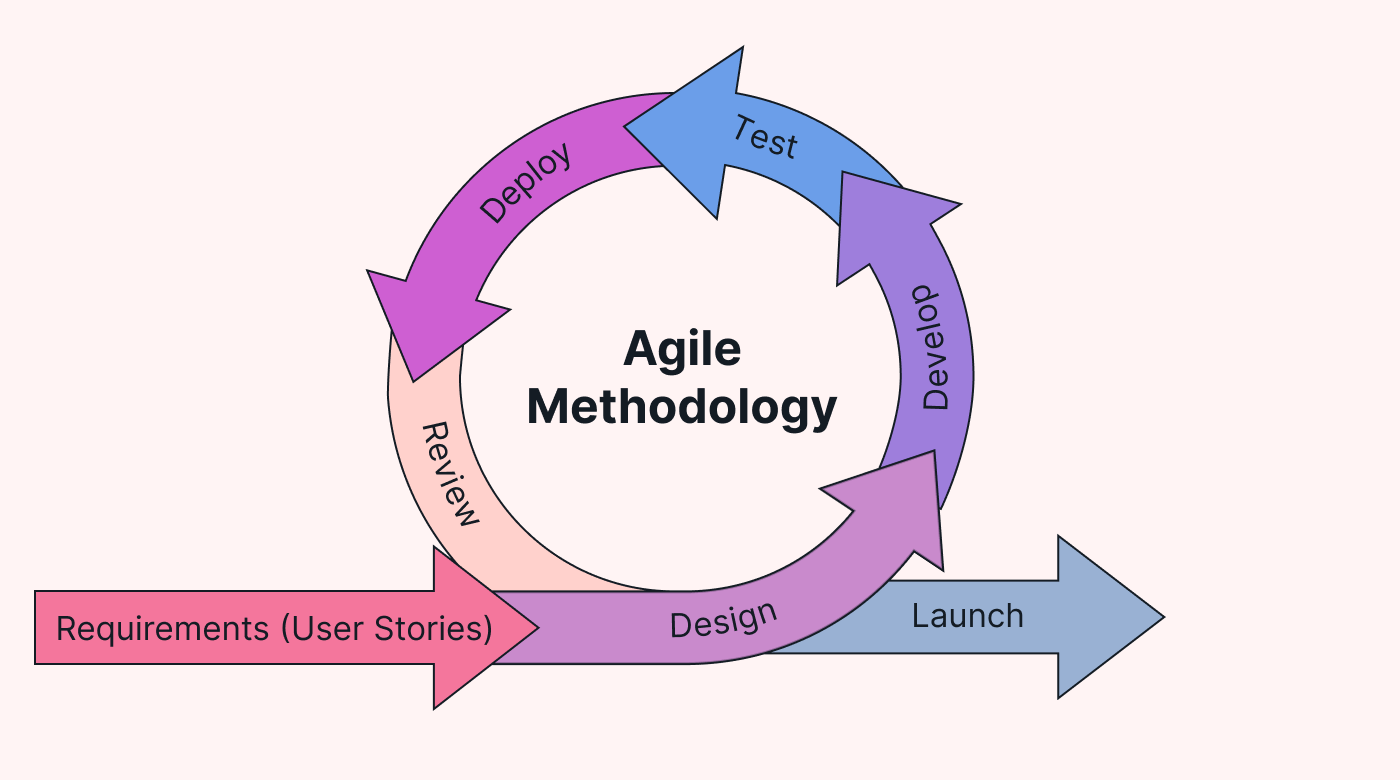
\includegraphics[width=0.95\textwidth]{assets/chapter1/agile_methodology.png}
\caption{Agile Scrum Methodology Workflow}
\label{fig:agile-methodology}
\end{figure}

\subsubsection{Characteristics of Agile Scrum}

\textbf{Sprint-Based Delivery:} The IoT-REAP project is organized into fixed 2-week sprints, each with a clear starting point (Sprint Planning), daily synchronization (Daily Standup), and endpoint (Sprint Review \& Retrospective). This structure provides predictable delivery cycles and regular stakeholder engagement.

\textbf{Sprint Planning \& Commitment:} At the beginning of each sprint, the team (in the solo developer context, this involves supervisors and stakeholders) commits to specific user stories and tasks. Sprint planning defines clear acceptance criteria, ensuring understanding of requirements before development begins.

\textbf{Product Backlog Management:} Features and requirements are maintained in a prioritized Product Backlog of 50 user stories (245 story points total). The Product Owner role prioritizes items based on business value, risk, and dependencies. This allows adaptation: new security requirements or infrastructure changes are incorporated into subsequent sprints.

\textbf{Sprint Increments:} Each sprint produces a working increment of the software. Early sprints deliver authentication and VM provisioning; middle sprints add remote desktop and robot control; later sprints implement AI scheduling and compliance features. This incremental approach enables early validation through the Sprint 3 MVP demo.

\textbf{Daily Standups \& Transparency:} Regular synchronization meetings (adapted to weekly supervisor meetings in this solo context) maintain transparency on progress, blockers, and dependencies. This enables rapid problem-solving and prevents misalignment.

\textbf{Sprint Review \& Stakeholder Feedback:} At each sprint boundary, completed work is demonstrated to stakeholders. This enables immediate validation, ensures features meet needs, and allows requirement refinement for subsequent sprints.

\textbf{Sprint Retrospective \& Process Improvement:} After each sprint review, the team conducts retrospectives to identify what goes well, what can improve, and what to change. This continuous improvement mindset enhances developer productivity, code quality, and stakeholder satisfaction over successive iterations.

\textbf{Definition of Done:} Scrum requires clear acceptance criteria for task completion. For IoT-REAP, "done" means: code written, unit tests passing (target 80\% coverage), code reviewed against project guidelines, feature documented, and acceptance criteria validated.

\subsection{Product Backlog}

The IoT-REAP platform development followed Agile Scrum principles with a prioritized product backlog organized by sprint. The complete backlog comprises 50 user stories totaling 245 story points. Table \ref{tab:product-backlog} presents key user stories with priorities and sprint assignments.

\begin{longtable}{|p{0.03\textwidth}|p{0.70\textwidth}|p{0.08\textwidth}|p{0.09\textwidth}|}
\caption{IoT-REAP Platform Product Backlog}
\label{tab:product-backlog} \\
\hline
\textbf{ID} & \textbf{User Story / Feature} & \textbf{Priority} & \textbf{Sprint} \\
\hline
\endfirsthead

\multicolumn{4}{c}{\tablename\ \thetable} \\
\hline
\textbf{ID} & \textbf{User Story / Feature} & \textbf{Priority} & \textbf{Sprint} \\
\hline
\endhead

\hline
\endfoot

\hline
\endlastfoot

\multicolumn{4}{|c|}{\textbf{Sprint 1: Foundation \& Authentication (26 SP)}} \\
\hline
01 & As a user, I want to register and log in securely using session-based authentication & High & Sprint 1 \\
\hline
02 & As an admin, I want role-based access control (engineer, admin, security\_officer) & High & Sprint 1 \\
\hline
03 & As a developer, I need database schema for users with ULID primary keys & High & Sprint 1 \\
\hline
04 & As a user, I want password reset functionality via email & Medium & Sprint 1 \\
\hline
05 & As a developer, I need React frontend with TypeScript and Zustand state management & High & Sprint 1 \\
\hline
\multicolumn{4}{|c|}{\textbf{Sprint 2: Proxmox Integration (28 SP)}} \\
\hline
06 & As a developer, I need database schema for VM nodes, templates, and sessions & High & Sprint 2 \\
\hline
07 & As a developer, I need Proxmox API client with retry logic and error handling & High & Sprint 2 \\
\hline
08 & As an engineer, I want to browse VM templates and launch sessions & High & Sprint 2 \\
\hline
09 & As a developer, I need load balancer to distribute VMs across Proxmox nodes & High & Sprint 2 \\
\hline
10 & As an admin, I want to view all nodes with live CPU/RAM stats & Medium & Sprint 2 \\
\hline
11 & As an admin, I want to register multiple Proxmox servers with encrypted credentials & High & Sprint 2 \\
\hline
\pagebreak[4]
\multicolumn{4}{|c|}{\textbf{Sprint 3: Guacamole Remote Access — MVP (26 SP)}} \\
\hline
12 & As a developer, I need Guacamole client service for connection management & High & Sprint 3 \\
\hline
13 & As an engineer, I want browser-based RDP/VNC access to my VM session & High & Sprint 3 \\
\hline
14 & As an engineer, I want to extend my session duration (+30 min increments) & High & Sprint 3 \\
\hline
15 & As an engineer, I want to terminate my session and have the VM cleaned up & High & Sprint 3 \\
\hline
16 & As an engineer, I want to save my preferred connection settings (display, audio) & Medium & Sprint 3 \\
\hline
\multicolumn{4}{|c|}{\textbf{Sprint 4: File Transfer \& Robot Foundation (28 SP)}} \\
\hline
17 & As a developer, I need MQTT service for robot command publishing & High & Sprint 4 \\
\hline
18 & As an engineer, I want to reserve a robot with atomic transaction locks & High & Sprint 4 \\
\hline
19 & As an engineer, I want to control the robot using Blockly visual programming & High & Sprint 4 \\
\hline
20 & As an engineer, I want an emergency stop button that works instantly & High & Sprint 4 \\
\hline
21 & As an engineer, I want real-time robot telemetry via WebSocket & High & Sprint 4 \\
\hline
\multicolumn{4}{|c|}{\textbf{Sprint 4.5: Technical Training Platform (45 SP)}} \\
\hline
41 & As an instructor, I want to create structured courses with modules, lessons, and prerequisite tracking & High & Sprint 4.5 \\
\hline
42 & As an instructor, I want to upload videos with HLS streaming and multi-quality playback (360p-1080p) & High & Sprint 4.5 \\
\hline
43 & As a learner, I want to enroll in courses and track my progress across lessons and modules & High & Sprint 4.5 \\
\hline
44 & As an instructor, I want to create timed quizzes with auto-grading, passing scores, and retry limits & High & Sprint 4.5 \\
\hline
45 & As a learner, I want hands-on VM lab sessions integrated with course lessons for practical training & High & Sprint 4.5 \\
\hline
46 & As a learner, I want to receive verifiable digital certificates upon course completion & High & Sprint 4.5 \\
\hline
47 & As a learner, I want to take timestamped notes during video lessons for later review & Medium & Sprint 4.5 \\
\hline
48 & As a learner, I want to rate and review courses to help other learners & Medium & Sprint 4.5 \\
\hline
49 & As an instructor, I want analytics dashboard showing enrollments, completions, and revenue & High & Sprint 4.5 \\
\hline
50 & As an admin, I want to manage course categories and featured course placement & Medium & Sprint 4.5 \\
\hline
\multicolumn{4}{|c|}{\textbf{Sprint 5: Camera \& AI Scheduler (34 SP)}} \\
\hline
22 & As a developer, I need Python FastAPI microservice for ML demand forecasting & High & Sprint 5 \\
\hline
23 & As an admin, I want 24-hour VM demand predictions with auto-refresh & High & Sprint 5 \\
\hline
24 & As a developer, I need idle session hibernation (suspend after 10 min inactivity) & Medium & Sprint 5 \\
\hline
25 & As an engineer, I want live camera feed from ESP32-CAM during robot control & High & Sprint 5 \\
\hline
\multicolumn{4}{|c|}{\textbf{Sprint 6: Zero-Trust Security — Feature Complete (34 SP)}} \\
\hline
26 & As a developer, I need device fingerprinting service & High & Sprint 6 \\
\hline
27 & As a developer, I need geo-IP anomaly detection using MaxMind & High & Sprint 6 \\
\hline
28 & As a security officer, I want real-time risk scores (0-100) for all sessions & High & Sprint 6 \\
\hline
29 & As a security officer, I want automatic session termination when risk > 85 & High & Sprint 6 \\
\hline
30 & As a developer, I need predictive maintenance AI for robot health scoring & High & Sprint 6 \\
\hline
\pagebreak[4]
\multicolumn{4}{|c|}{\textbf{Sprint 7: OT Isolation, Catalog \& Compliance (34 SP)}} \\
\hline
31 & As an admin, I want to enforce Purdue model network isolation (IT/OT zones) & High & Sprint 7 \\
\hline
32 & As a developer, I need tamper-proof audit log with SHA-256 hash chain & High & Sprint 7 \\
\hline
33 & As an admin, I want PDF compliance reports for IEC 62443 audits & High & Sprint 7 \\
\hline
34 & As an engineer, I want AI-assisted template suggestions based on my description & Medium & Sprint 7 \\
\hline
35 & As an admin, I want complete dashboard with quota management and activity logs & High & Sprint 7 \\
\hline
\multicolumn{4}{|c|}{\textbf{Sprint 8: Testing(35 SP)}} \\
\hline
36 & As a developer, I need 80\% test coverage with mocked external APIs & High & Sprint 8 \\
\hline
37 & As a developer, I need load testing: 50 concurrent logins, 25 VMs, 40 Guacamole sessions & High & Sprint 8 \\
\hline
38 & As a security officer, I need OWASP ZAP scan with 0 critical/high findings & High & Sprint 8 \\
\hline
39 & As a user, I want comprehensive documentation (user manual, API docs) & High & Sprint 8 \\
\hline
40 & As a developer, I need to prepare and deliver 15-minute live demo & High & Sprint 8 \\
\hline
\end{longtable}

\subsection{Agile Scrum Ceremonies and Collaboration}

\textbf{Sprint Planning (Duration: 2-4 hours):} At the beginning of each 2-week sprint, sprint planning meetings engage the developer, supervisors, and Advisory Unit stakeholders. Sessions define sprint goals, select user stories from the prioritized Product Backlog (based on business value and dependencies), and break them into implementation tasks. Each user story receives effort estimation using story points, resulting in a Sprint Backlog of committed work with clear acceptance criteria. This ceremony ensures shared understanding of requirements and realistic commitment.

\textbf{Daily Standup (Duration: 15 minutes):} Although conducted as a solo developer, daily progress tracking maintains transparency. Weekly formal standups (Mondays) with supervisors answer three questions: What was completed? What will be done? What obstacles exist? This adaptation of the daily ceremony pattern provides checkpoint accountability while respecting the solo context.

\textbf{Sprint Review \& Demo (Duration: 1-2 hours):} At each sprint's end, completed work is demonstrated to stakeholders. Reviewers examine running features, validate acceptance criteria compliance, and provide feedback influencing subsequent sprint prioritization. The Sprint 3 review includes a formal MVP (Minimum Viable Product) demo showcasing VM provisioning, remote desktop access, and basic robot control—a critical milestone confirming core platform viability.

\textbf{Sprint Retrospective (Duration: 1 hour):} Following the review, the team conducts retrospectives examining what works well, what can improve, and specific action items for the next sprint. Early retrospectives identify: need for more comprehensive API documentation, benefit of Copilot-assisted development, and infrastructure bottlenecks requiring architectural adjustments. These insights are systematically incorporated into subsequent sprints, improving productivity and code quality.

\textbf{Product Backlog Refinement (Ongoing):} Between sprints, the Product Backlog is continuously refined. New requirements (additional security measures, infrastructure changes, performance optimizations) are added, prioritized, and estimated. This preparation ensures Sprint Planning sessions are efficient and focused on high-value items.

\subsection{The UML Modeling Language}

\begin{figure}[H]
\centering

\includegraphics[width=8cm]{assets/chapter1/uml.png}
\caption{UML modeling language}
\label{fig:uml-logo}
\end{figure}

Unified Modeling Language (UML) is a standardized visual modeling language used in software engineering to specify, visualize, construct, and document the artifacts of software systems \cite{booch2005}. Developed by Grady Booch, James Rumbaugh, and Ivar Jacobson in the mid-1990s, UML provides a common vocabulary for object-oriented software design and is the industry standard for software architecture documentation.

UML consists of multiple diagram types that capture different aspects of system design:

\begin{itemize}
    \item \textbf{Structural Diagrams:} Class diagrams, component diagrams, deployment diagrams, package diagrams
    \item \textbf{Behavioral Diagrams:} Use case diagrams, sequence diagrams, activity diagrams, state machine diagrams
\end{itemize}

For the IoT-REAP platform development, UML modeling provided a visual framework for communicating system architecture, clarifying requirements, and documenting design decisions across the development team and stakeholders.

\section{Project Planning}

The IoT-REAP platform development is organized as a phased timeline from February to mid-June 2026, following an Agile Scrum sprint-based approach \cite{agile}. The project is structured into eight two-week sprints with a small integration and testing buffer, and it reaches two key milestones at Sprint 3 (MVP Demo) and Sprint 6 (Feature Complete).

\subsection{Sprint-Based Development Phases}

The following phases present the project timeline in chronological order, showing how the platform evolved from foundation and integration work to testing and final delivery.

\textbf{Sprint 1: Foundation \& Authentication (February 2-15, 2026)}

Establishes project foundation with Laravel 12 and React 18 integration via Breeze. Implements session-based authentication, role-based access control (engineer, admin, security\_officer), and database schema with ULID primary keys. Sets up MySQL, Redis, and Docker development environment.

\textbf{Sprint 2: Proxmox Integration (February 16 - March 1, 2026)}

Builds Proxmox VE API client wrapper with retry logic and error handling. Creates database schema for VM nodes, templates, and sessions. Implements load balancer for VM distribution across nodes and admin node management dashboard with live stats.

\textbf{Sprint 2.5: Multi-Proxmox Server Support (March 2-8, 2026)}

Extends architecture to support multiple independent Proxmox clusters. Implements encrypted credential storage, server registration API, and cluster selection logic for engineers launching VMs.

\textbf{Sprint 3: Guacamole Remote Access — MVP Demo (March 9-22, 2026)}

Deploys Apache Guacamole and integrates its API with Laravel. Implements connection creation, one-time token generation, and embedded viewer in React. Adds session extension, termination, and connection preference persistence. \textbf{This sprint culminates in the MVP demonstration.}

\textbf{Sprint 4: File Transfer \& Robot Foundation (March 23 - April 5, 2026)}

Builds MQTT infrastructure for robot command publishing with QoS 1. Creates atomic robot reservation system preventing double-booking. Deploys Blockly visual programming interface and implements real-time telemetry streaming via WebSocket.

\textbf{Sprint 4.5: Technical Training Platform (April 6-19, 2026)}

Develops comprehensive learning management system for industrial skills training. Implements course structure with modules, lessons (video, reading, practice, VM-lab types), and prerequisite tracking. Builds HLS video streaming with adaptive quality (360p-1080p) and progress tracking. Creates timed quiz system with auto-grading, passing scores, and retry limits. Integrates VM lab sessions directly into course lessons for hands-on practice. Implements digital certificate generation with unique verification hashes.

\textbf{Sprint 5: Camera \& AI Scheduler (April 20 - May 3, 2026)}

Deploys Python FastAPI microservice for ML-based demand forecasting using RandomForestRegressor. Integrates predictions with Laravel scheduler for VM pre-warming. Adds live ESP32-CAM video feed and idle session hibernation.

\textbf{Sprint 6: Zero-Trust Security — Feature Complete (May 4-17, 2026)}

Implements device fingerprinting and geo-IP anomaly detection. Builds real-time risk scoring engine with automatic session termination for high-risk activities. Trains IsolationForest model for robot health anomaly detection. \textbf{All core backlog items are implemented at this checkpoint.}

\textbf{Sprint 7: OT Isolation, Catalog \& Compliance (May 18-31, 2026)}

Enforces Purdue model network isolation with IT/OT zone separation. Builds tamper-proof audit log with SHA-256 hash chain for IEC 62443 compliance. Implements PDF compliance report generator and AI-assisted template catalog.

\textbf{Sprint 8: Testing(June 1-14, 2026)}

Achieves 80\% test coverage with mocked external APIs. Conducts load testing (50 concurrent logins, 25 VMs, 40 Guacamole sessions). Executes OWASP ZAP security scan. Prepares documentation and rehearses defense presentation.

\begin{figure}[H]
\centering
\rotatebox{-90}{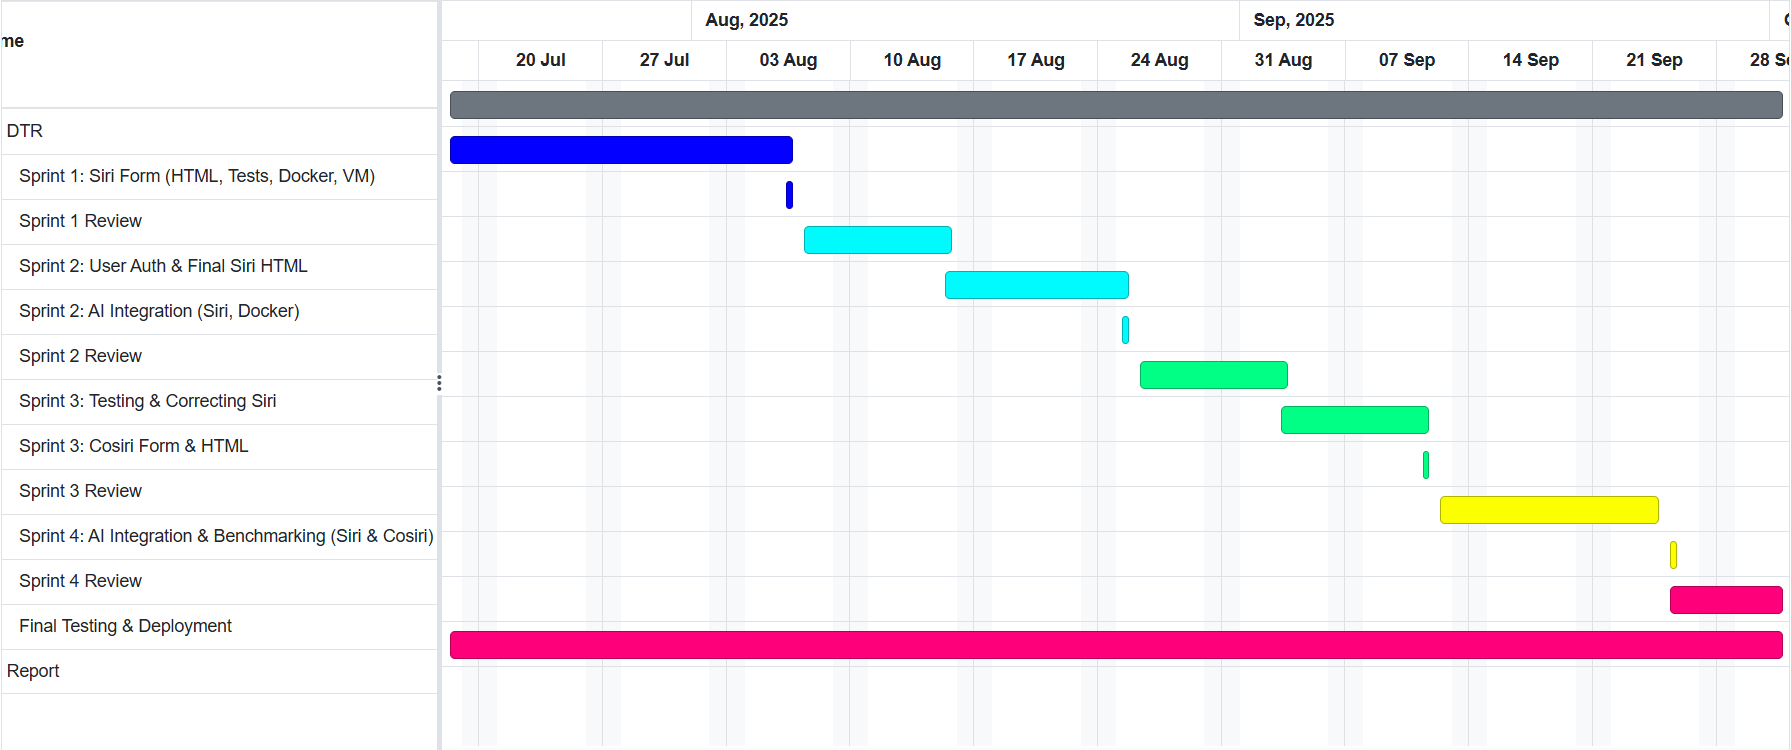
\includegraphics[width=23cm]{assets/chapter1/gantt.png}}
\caption{IoT-REAP Platform Development Timeline and Milestones (need to be changed)}
\label{fig:project-timeline}
\end{figure}

\section*{Conclusion}
\addcontentsline{toc}{section}{Conclusion}

This chapter established the project context, studied current remote access limitations, presented the IoT-REAP solution, specified the main requirements, and described the Agile Scrum methodology and sprint planning used to organize the work.

\cleardoublepage

